\documentclass[10pt]{article}
\usepackage[utf8]{inputenc}
\usepackage[spanish]{babel}

%Fuente (compilarlo en Latex.pdf normal porque va más rápido y luego
%y al final insertarlo en Arial) DA ERROR
%\usepackage{fontspec}
%\setmainfont{Arial}

%Estructura de la Página
\usepackage[left=2.54cm,right=2.54cm,top=2.54cm,bottom=2.54cm]{geometry}

%Páginas en horizontal


%Pies de página y encabezado
\usepackage{fancyhdr}

%Comentario párrafos
\usepackage{verbatim}

%Paquete arquitectura página
\pagestyle{fancy}
\fancyhf{}
\lhead{José Honrubia Blanco}
\rhead{Exámenes Mecánica de Máquinas}
\rfoot{\thepage}
\lfoot{Academia David Martínez}

%Interlineado
\renewcommand{\baselinestretch}{1}



%Paquete Matemático
\usepackage{amsmath}
\usepackage{amsfonts}
\usepackage{amssymb}
\usepackage{breqn}

%Paquete para el código
% Paquetes Listing

\usepackage{listings}
\usepackage{xcolor}

%Settings 

\definecolor{codegreen}{rgb}{0,0.6,0}
\definecolor{codegray}{rgb}{0.5,0.5,0.5}
\definecolor{codepurple}{rgb}{0.58,0,0.82}
\definecolor{backcolour}{rgb}{0.95,0.95,0.92}


\lstdefinestyle{mystyle}{
 backgroundcolor=\color{backcolour},   
 commentstyle=\color{codegreen},
 keywordstyle=\color{magenta},
 numberstyle=\tiny\color{codegray},
 stringstyle=\color{codepurple},
 basicstyle=\ttfamily\footnotesize,
 breakatwhitespace=false,         
 breaklines=true,                 
 captionpos=b,                    
 keepspaces=true,                 
 numbers=left,                    
 numbersep=5pt,                  
 showspaces=false,                
 showstringspaces=false,
 showtabs=false,                  
 tabsize=2
}

\lstset{style=mystyle}
%Paquete Imágenes
\usepackage{wrapfig}
\usepackage{graphicx}
\usepackage{subcaption}
\graphicspath{ {imagenes/} }



%Bibliografía
\usepackage[backend=bibtex]{biblatex}
\addbibresource{referencias.bib}

%Espacio entre párrafos
\setlength{\parskip}{0.02cm}
%Sangría
\setlength{\parindent}{0cm}




\title{Examen 1 Mecánica de Maquinas}
\author{José Honrubia Blanco }
\date{Noviembre 2022}

\begin{document}

\section{Examen 2}
\textbf{Problema 1}. (1.5 puntos) La unidadd de bombeo que se muestra en la figura se emplear para extraer petróleo. Cuando la viga de balancín ABC está en posición horizontal, la fuerza \textbf{P} que actúa en el cable de perforación situado en la cabeza del pozo es de 200 kN. La cabeza de aballo C pesa 60 kN y su centro de gravedad se encuentra en $G _{C}$. La viga balancín ABC tiene un peso de 130 kN y su centro de gravedad ubicado en $G _{B}$, y el contrapeso tiene un peso de 200 kN y el centro de gravedad en $G _{W}$. La biela AD está conectada mediante pasadores en sus extremos y tiene un peso despreciable. Para la posición mostrada:
\begin{itemize}
    \item Determine la fuerza ejercida por la biela AD. (0.5 p.)
    \item Determine el par \textbf{M} que debe ejercer el motor para vencer la carga suspendida en el cable de perforación (0.5 p.)
    \item Reduzca el sistema formado por la carga \textbf{P} del cable, los pesos de la viga de balancín y la cabeza de caballo y la fuerza ejercida por la biela AD a una única fuerza a lo largo de la línea ABC, e indique la coordenada del punto de aplicación de dicha fuerza con respecto del punot A en el caso de que sea posible la reducción. (0.5 p.)
\end{itemize}
\begin{figure}[h!]
    \centering
    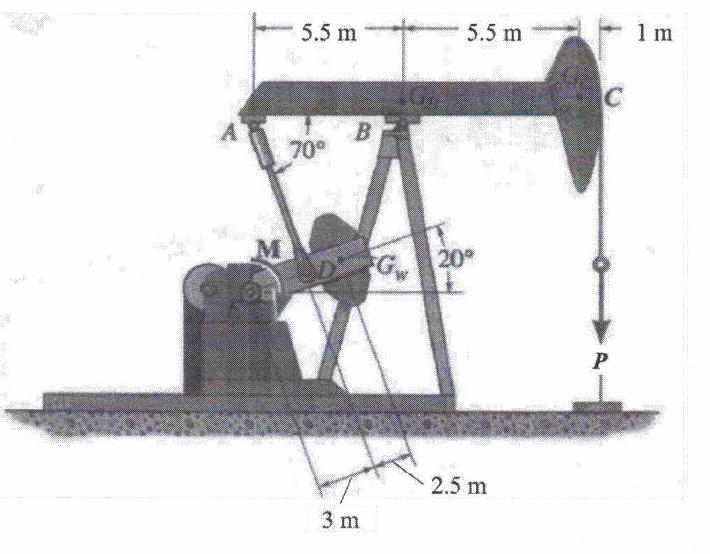
\includegraphics[width=0.45\linewidth]{problema_1.pdf}
    \label{fig:}
  \end{figure}
\\ 
\textbf{Problema 2}. (3 puntos) Para la superficie plana que se muestra en la figura, determine:

\begin{figure}[h!]
    \centering
    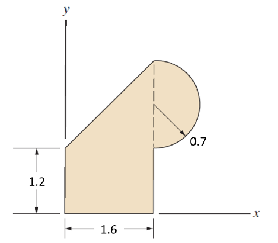
\includegraphics[width=0.35\linewidth]{problema_2.pdf}
  \label{fig:}
\end{figure}
\begin{itemize}
    \item Coordenadas de su centroide (según ejes de coordenadas mostrados). (0.5 p.)
    \item Momentos de inercia y producto de inercia de la sección mostrada respecto a lso ejes de coordenadas x e y mostrados. (0.75 p.)
    \item Momentoso y productos de inercia respecto a los ejes centroidales paralelos a los ejes x e y (0.75 p.)
    \item Parámetros (centro y radio) del círculo de Mohr para los momentos de inercia de los ejes centroidales. (0.25 p.)
    \item Represente lso valores obtenidos en el círculo de Mohr. Dibuje la orientación de los ejes principales respecto a lso ejes centroidales (trace las dierecciones de los ejes sobre la superficie). (0.25 p.)
    \item Superficie y volumen del sólido de revolución generado al rotar la geometría generatriz compeusta en el gráfico respecto al eje x. (0.5 p.)
\end{itemize}
\\
\textbf{Problema 3}. (1.5 puntos) El movimiento del cubo de la retroexcavadora que se muestra en la figura se controla mediante dos brazos y un eslabón articulado en D. Los brazos están colocados simétricamente respecto de los planos central, vertical y longitudinal de la restroexcavadora; en la figura sólo se muestra el brazo AFJ y su cilindro de control EF. El eslabón simple GHBD y su cilindo de control BC se encuentran localizados en el plano de simetría. Para la posición y la carga mostradas en la figura, determine la fuerza ejercida por:
\begin{itemize}
    \item El cilindro BC (0.5 p.)
    \item Cilindro EF (0.5 p.)
    \item Reacciones en A (0.5 p.)
\end{itemize}
\begin{figure}[h!]
    \centering
  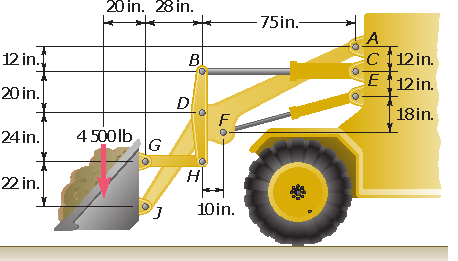
\includegraphics[width=0.45\linewidth]{problema_3.pdf}
  \label{fig:}
\end{figure}

\textbf{Problema 4}. (2 puntos) El ensamblaje mostrado en la figura se une al colarrín listo en el punto A, el cual se dispone sobre la barra vertical ubicada sobre el eje y. A su misma vez, el ensamblaje sostiene un letro de 50 kN de peso cuyo centro de gravedad se encuentra ubicado en G. Para las condiciones citadas:
\begin{figure}[h!]
    \centering
    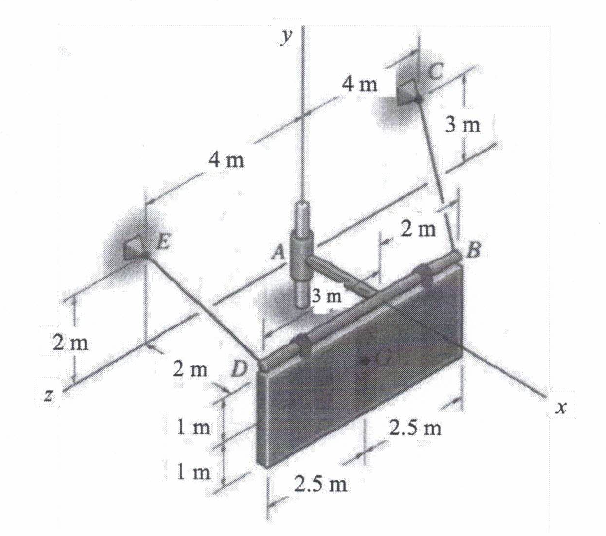
\includegraphics[width=0.45\linewidth]{problema_4.pdf}
    \label{fig:}
  \end{figure}
\begin{itemize}
    \item Dibuje el diagrama del sólido libre formado por el ensamblaje y el letrero (0.5 p.)
    \item Determine la tensión en cada uno de los cables (1 p.)
    \item Determine la reacción que actúa sobre el collarín (fuerza y par) (0.5 p.)
    \item Reduzca el sistema formado por las tensiones y el peso del letrero a un sistema equivalente fuerza-par en el punto A (0.5 p.)
\end{itemize}

\textbf{Problema 5}. (2 puntos) Los pesos de las cajas mostradas en laf igura son $W _{A}$ = 200 N y $ W _{B}$ = 700 N, respectivamente. El coeficiente de fricción estática entre las cajas A y B y entre la caja B y el suelo es 0.12. La polea tiene un radio de 100 mm y está montado sobre un eje de 20 mm. Calcular:
\begin{itemize}
    \item La fuerza máxima F que se puede aplicar para que las cajas no deslicen suponiendo que el coeficiente de fricción entre el eje y la polea y entre la cuerad y la polea es nulo. Calcule también la tensión en la cuerda (0.5 p)
    \item Calcule la fuerza ma´xima F que se puede aplicar para que las cajas no deslicen suponiendo el coeficiente de rozamiento entre la cuerda y la polea es de 0.15. Calcule la tensión en la cuerda (0.75 p).
    \item ¿Qué ocurriría con la tensión en la cuerda si existiera un coeficiente de fricción entre el eje de la polea? Justifique su respuesta indicando el por qué de la imsma. Plantee las ecuaciones del sistema necesarias para calcular el valor de la fuerza F para que las cajas no deslicen y la tensión en la cuerda considerando además del coeficiente de fricción entre ambas cajas y la caja B y el suelo de 0.12, un coeficiente de fricción de 0.16 en el eje de l apolea. Para este apartado considere que la fricción entre la cuerda y la polea es despreciable. (0.75 p.)
\end{itemize}
\begin{figure}[h!]
  \centering
  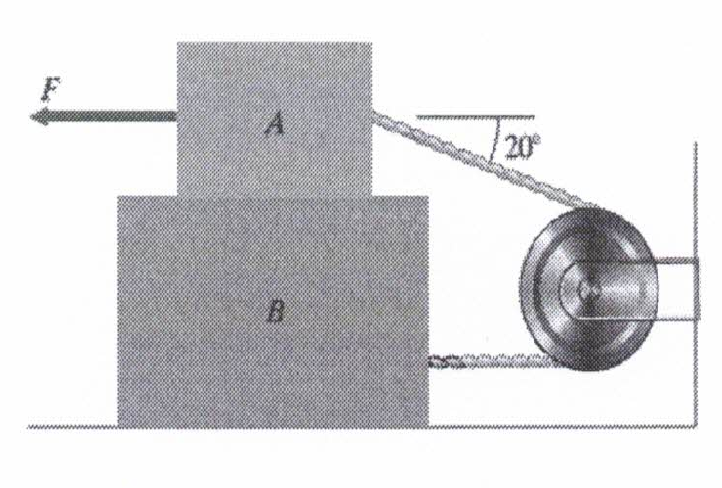
\includegraphics[width=0.45\linewidth]{problema_5.pdf}
  \label{fig:}
\end{figure}

\end{document}